\begin{center}
  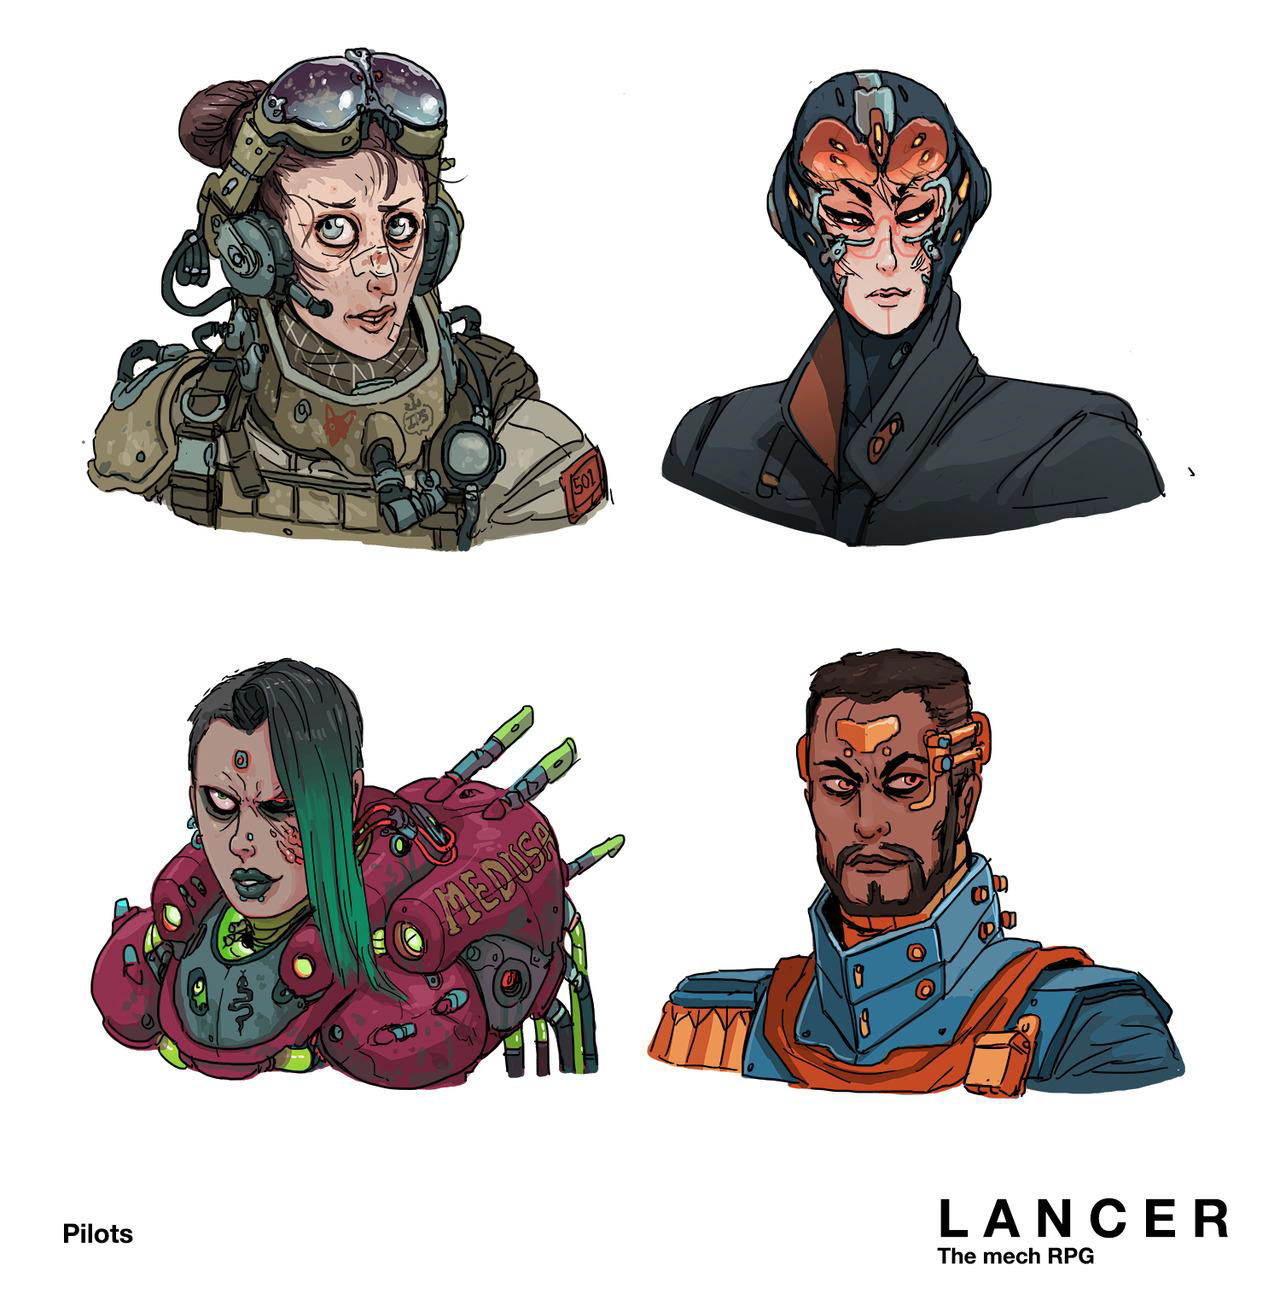
\includegraphics{Pilots2}
\end{center}

\chapter{The Basic Structure of Lancer: Narrative Play}

LANCER as a game is focused on the \textbf{mission.} The most important thing about a mission is there are some \textbf{stakes} involved. There’s something that needs doing, and probably needs doing fast! There’s natural tension in the story that needs to be resolved through player action, and without the players intervening, the outcome will be radically different (often for the worse!). If you’re not on a mission, you’re in \textbf{downtime.} During downtime, the moment-to-moment action is probably not as important, and things can ‘montage’ or jump from scene to scene quite easily. There’s often less tension or time sensitivity (but not necessarily none at all).

Any given story of LANCER always begins in downtime, unless it’s the first session. If it’s the first session, see the section below!

During downtime, players do the following:\\
-   Take \textbf{downtime actions} to work on personal projects to progress the story or gain \textbf{reserves} (more on that shortly)\\
-   Play out any other freeform scenes between the players or NPCs

Downtime lasts until the next mission. Before a mission starts, the following steps take place:\\
- \textbf{Brief} - The players or the GM establish what the \textbf{goal} of the mission is, and the GM establishes the \textbf{stakes.}\\
- \textbf{Preparation} - Players choose the mech they are going to start with for this mission, pick pilot gear, establish reserves, and make any other preparations\\
- \textbf{Boots on the Ground} - We cut to the players right as they arrive on the scene.

When the mission is over (completed or abandoned or resolved in one way or another -even negatively!), players can \textbf{debrief, level up,} and return to downtime. The loop then continues.

The following sections will explain each step in a little more detail. We’ll go in the order you’d usually go during your first session

                                               \textbf{The first session} 

During the first session, it’s recommended to skip right over downtime and go right to the\textbf{brief} and onwards. You’ll also want to take the extra step of establishing \textbf{who we are} with the players, if you haven’t already. Some GMs and players already have a good idea of what this is before coming to the table, but it’s perfectly fine to start the first session without having anything firmly established. Many groups even play through a first session in order to establish who their group is and don’t want to establish it before they start- that’s fine too.

However, establishing a common goal or purpose before the end of the first session will definitely help with explaining character motivation and cohesion. If you need inspiration you can roll on the tables below or establish it with your group.

\textbf{TABLE: Who are we?}

 d20       Identity

 1         An infamous private military corporation

 2         Glory-seeking warriors

 3         Union Regulars, career soldiers

 4         Union Auxiliaries, recruited from a local world

 5         Elites of the Planetary Defense Force

 6         Enforcers of the Law

 7         Criminals, Thieves, and Swindlers

 8         Acolytes of an ancient martial order

 9         Devotees of a higher power

  10       Guardians of an ancient royal lineage

  11       Corporate security, asset protection

  12       Explorers of the unknown

  13       Pirate scum

  14       Defenders of the homeland

  15       The forefront of the rebellion

  16       Saviors of the weak and helpless

  17       Hungry travelers, in it for the money

  18       Inventors, engineers, and test subjects

  19       Inheritors of a famous legacy

  20       The only ones who can stop what’s coming

If your players have a patron or a parent organization, you can establish that here

\textbf{TABLE: Who gives us orders?}

 d20       Patron

 1-2       Anyone who pays us

 3-4       Our commanding officer

 5-6       The Hierophant or high priest

 7-8       A corporate patron or sponsor

 9-10      Our ancient martial code or law, our duty

 11-12     Our mentor and founder

 13-14     Our local Union Administrator and high command

 15-16     The whisperings of a long-dead monolith

 17-18     Our liege lord or king

 19-20     The elders of our organization

Finally, if you want to establish some history or relationships between the players, you can do
that quickly and easily. Go around the table and ask each player to choose exactly one or two
other players and ask them to establish one quick fact or experience that the two characters
have between them. If you like, and you have time, you can play out a scene or two to get a
good feeling of the characters.

You can use the questions on the table below as prompts. A player can ask one or two of these
to the table in general and write down answers. Nobody has to answer any question, especially if
they don’t know the answer yet or the question makes them uncomfortable. Remember to be
respectful of your fellow players!

\textbf{TABLE: Personal History}

 d20       Personal	History

 1         Which of you did I grow up with?

 2         Which of you almost killed me once?

 3         Which of you was I in love with (or still am)?

 4         Which have you have I served with for some time?

 5         Which of you distrusts me?

 6         Which of you have I gotten drunk with more than once?

 7         Which of you sees me as a mentor?

 8         Which of you taught me all I know about building mechs?

 9         Which of you was I marooned with on a hostile planet for some time?

10       Which of you took me on my first mission?

  11       Which of you is most likely to ask me for advice?

  12       Which of you knows a deep secret of mine? What is it?

  13       Which of you thinks they have me all figured out?

  14       Which of you finds me completely incomprehensible?

  15       Which of you is the most curious about me?

  16       Which of you finds me attractive?

  17       Which of you thinks they can teach me a thing or two?

  18       Which of you never expected to see me again?

  19       Which of you will support and stand by me, no matter what?

  20       Which of you calls me a friend?

Adding personal history between the character adds hooks and relationships that can influence
how characters treat each other and creates fun roleplaying opportunities. It’s perfectly fine to
start without any history between characters if that’s how you prefer to play your game.

\subimport{./basicStructure/}{brief}

\subimport{./basicStructure/}{preparation}

\subimport{./basicStructure/}{boots}

\subimport{./basicStructure/}{narrative}

\subimport{./basicStructure/}{debrief}

\subimport{./basicStructure/}{downtime}
